\newcommand{\BEDD}{BEDD\xspace}
\newcommand{\fignatA}{/home/robin/RECHERCHE/RESEAUX/GOF-Network/Motif_Analysis_Natasha/Figures}
\newcommand{\fignatB}{/home/robin/RECHERCHE/RESEAUX/GOF-Network/Motif_Analysis_Natasha/Article/Figures}
\newcommand{\tabnat}{/home/robin/RECHERCHE/RESEAUX/EXPOSES/2504-Montpellier/Tables}

%==================================================================
%==================================================================
\subsection{Bipartite networks and motifs}
% \frame{\frametitle{Outline} \tableofcontents[currentsubsection]}
%==================================================================
\frame{\frametitle{Bipartite network}

  \begin{tabular}{ll}
    \begin{tabular}{p{.45\textwidth}}
      \paragraph{Two types of actors.}
      \begin{itemize}
      \item Mutualistic: plant-pollinator
      \item Antagonistic: host-parasite
      \end{itemize}
      \bigskip \bigskip 
      \paragraph{Topological analysis:} \\
      understanding the network organisation \\
      \bigskip
      \paragraph{Local:} % \\
      node or edge properties (degree, betweenness) \\
      \bigskip
      \paragraph{Global:} % \\
      density, connected components, nestedness 
    \end{tabular}
    &
    \begin{tabular}{p{.45\textwidth}}
      \paragraph{Zackenberg network: } 
      \refer{SRO16} \\
      \includegraphics[width=.4\textwidth, trim=0 50 0 50]{\fignet/Zackenberg-1996_12-red-net} \\
%       \includegraphics[width=.4\textwidth, trim=0 50 0 50]{\fignet/Zackenberg-1996_12-red-adj}
    \end{tabular} 
  \end{tabular}
}

%==================================================================
\frame{\frametitle{Bipartite network: data}

  \begin{tabular}{ll}
    \begin{tabular}{p{.6\textwidth}}
      \paragraph{Species.}
      \begin{itemize}
        \setlength{\itemsep}{.75\baselineskip}
        \item $i = 1, \dots m$ pollinators = rows = bottom nodes
        \item $j = 1, \dots n$ plants = columns = top nodes
      \end{itemize}
    \end{tabular}
    &
    \hspace{-.15\textwidth}
    \begin{tabular}{p{.4\textwidth}}
      \includegraphics[width=.4\textwidth, trim=0 50 0 50]{\fignet/Zackenberg-1996_12-red-net} 
    \end{tabular} 
    \\ \pause
    \begin{tabular}{p{.6\textwidth}}
      \paragraph{Interactions.}
      \begin{itemize}
      \item $Y_{ij} = 1$ if pollinator $i$ interacts with plant $j$, \\
      0 otherwise
      $$
      Y_{ij} = 1 \quad \Leftrightarrow \quad i \sim j
      $$
      \item adjacency matrix : $m \times n$
      $$
      Y = [Y_{ij}]_{1 \leq i \leq m, 1 \leq j \leq n}
      $$
      \end{itemize}
    \end{tabular}
    &
    \hspace{-.15\textwidth}
    \begin{tabular}{p{.5\textwidth}}
      \includegraphics[width=.4\textwidth, trim=0 50 0 50]{\fignet/Zackenberg-1996_12-red-adj}
    \end{tabular} 
  \end{tabular}
}

%==================================================================
\frame{\frametitle{Bipartite motifs}

  \label{sec:motifList}
  \begin{tabular}{ll}
    \hspace{-.04\textwidth}
    \begin{tabular}{p{.45\textwidth}}
      \paragraph{'Meso-scale' analysis.} \refer{SCB19}
      \begin{itemize}
       \item Motifs ='building-blocks'
       \item between local (several nodes) and global (sub-graph)
      \end{itemize}
      \bigskip \bigskip 
      \onslide+<2->{
      \paragraph{Interest.}
      \begin{itemize}
       \item Generic description of a network
       \item Enables network comparison
       \item Even when the nodes are different
      \end{itemize} \\
      \textcolor{gray}{($+$ 'species-role': out of the scope here)} \\
      }
    \end{tabular}
    &
    \begin{tabular}{p{.45\textwidth}} 
      \hspace{-0.035\textwidth}
      \includegraphics[width=.45\textwidth]{\fignet/SCB19-Oikos-Fig3-6motifs} \\      
    \end{tabular} 
  \end{tabular}

  \bigskip \bigskip 
  \onslide+<3->{
  \paragraph{Existing tool.} 
  \url{bmotif} package \refer{SSS19}: 
  counts motif occurrences 
  (\emphase{Not an easy task!})
  }
  
}

%==================================================================
\frame{\frametitle{Example}

  \begin{tabular}{ll}
    \begin{tabular}{p{.45\textwidth}}
      \paragraph{Plant-pollinator network} \refer{SRO16} \\
      \hspace{-.05\textwidth}
      \includegraphics[width=.45\textwidth, trim=0 50 0 50]{\fignet/Zackenberg-1996_12-red-net} \\
    \end{tabular}
    &
    \begin{tabular}{p{.45\textwidth}}
      \paragraph{Motif counts.}  \\ ~\\ 
      4 nodes (species) \\ 
      \includegraphics[width=.09\textwidth]{\fignet/Zackenberg-1996_12-red-motif5} 
      \includegraphics[width=.09\textwidth]{\fignet/Zackenberg-1996_12-red-motif6} \\ ~\\
      5 nodes \\ 
      \includegraphics[width=.09\textwidth]{\fignet/Zackenberg-1996_12-red-motif9} 
      \includegraphics[width=.09\textwidth]{\fignet/Zackenberg-1996_12-red-motif10} 
      \includegraphics[width=.09\textwidth]{\fignet/Zackenberg-1996_12-red-motif11} 
      \includegraphics[width=.09\textwidth]{\fignet/Zackenberg-1996_12-red-motif12} \\
      \includegraphics[width=.09\textwidth]{\fignet/Zackenberg-1996_12-red-motif13} 
      \includegraphics[width=.09\textwidth]{\fignet/Zackenberg-1996_12-red-motif14} 
      \includegraphics[width=.09\textwidth]{\fignet/Zackenberg-1996_12-red-motif15} 
      \includegraphics[width=.09\textwidth]{\fignet/Zackenberg-1996_12-red-motif16} 
    \end{tabular}  
    ~ \\
    \hline
    \\ \pause
    \begin{tabular}{p{.45\textwidth}}
      top 'stars' (plants) \\
      \includegraphics[width=.09\textwidth]{\fignet/Zackenberg-1996_12-red-motif1} 
      \includegraphics[width=.09\textwidth]{\fignet/Zackenberg-1996_12-red-motif2} 
      \includegraphics[width=.09\textwidth]{\fignet/Zackenberg-1996_12-red-motif7} 
      \includegraphics[width=.09\textwidth]{\fignet/Zackenberg-1996_12-red-motif17} 
    \end{tabular}
    &    
    \begin{tabular}{p{.45\textwidth}}
      bottom 'stars' (pollinators) \\
      \includegraphics[width=.09\textwidth]{\fignet/Zackenberg-1996_12-red-motif1} 
      \includegraphics[width=.09\textwidth]{\fignet/Zackenberg-1996_12-red-motif3} 
      \includegraphics[width=.09\textwidth]{\fignet/Zackenberg-1996_12-red-motif4} 
      \includegraphics[width=.09\textwidth]{\fignet/Zackenberg-1996_12-red-motif8} 
    \end{tabular}
  \end{tabular}
  
}

%==================================================================
%==================================================================
\subsection{Expected degree distribution model}
\frame{\frametitle{Outline} \tableofcontents[currentsubsection]}
%==================================================================
\frame{\frametitle{NA null model}

  \bigskip 
  \paragraph{Motif counts} obviously depend on 
  \begin{itemize}
    \setlength{\itemsep}{.75\baselineskip}
    \item the \emphase{size} of the network: $n \times m$
    \item the \emphase{density} of the network
  \end{itemize}

  \bigskip \bigskip \pause
  \paragraph{A not-too-null} model also needs to account for the existence of generalists and specialists among both plants and pollinators
   
  \bigskip \bigskip \pause
  \paragraph{Bipartite expected degree distribution (\BEDD) model:} (literal version)
  \begin{itemize}
    \setlength{\itemsep}{.75\baselineskip}
    \item Each pollinator $1 \leq i \leq m$ has a specific \emphase{propensity to interact} (degree of generalism)
    \item Each plant $1 \leq j \leq n$ has a specific \emphase{propensity to interact}  (idem)
    \item The probability for pollinator $i$ and plant $j$ to interact is proportional to the \emphase{product of their respective propensities}.
  \end{itemize}

}

%==================================================================
\frame{\frametitle{Bipartite expected degree distribution (\BEDD) model}

  \paragraph{Model \refer{OLR22}:} \\~
  \begin{itemize}
    \setlength{\itemsep}{.75\baselineskip}
    \item \pause Latent variables $Z = (U, V)$: 
    $$
    (U_i)_{i = 1, \dots m}, (V_j)_{j = 1, \dots n} \text{ iid } \sim \Ucal[0, 1]
    $$
    \item \pause Observed variables $Y$
    $$
    (Y_{ij})_{1 \leq i \leq m, 1 \leq j \leq n} \text{ indep.} \mid Z:
    \quad Y_{ij} \mid U_i, V_i \sim \Bcal(\rho \; g(U_i) \; h(V_j))
    $$ 
    \item \pause Parameters $\theta = (\rho, g, h)$:
    \begin{align*}
      \rho & = \text{network density}, & 
      g & = \text{top node degree imbalance } \left(\int g = 1\right), \\
      & & h & = \text{bottom node degree imbalance } \left(\int h = 1\right)
    \end{align*}
  \end{itemize}
  
  \bigskip
  (Bipartite version of the EDD model \refer{ChL02})
  
}

%==================================================================
\frame{\frametitle{\BEDD model}

  \begin{tabular}{cccc}
    & & $h_0(v) =$ & $h(v) =$ \\
    \multicolumn{2}{c}{
      $\begin{array}{rl}
        \Pbb\{i \sim j \mid U_i, V_j\} & = \rho \; g(U_i) \; h(V_j) \\ \\
        \Esp (Y_{i+} \mid U_i) & = n \; \rho \; g(U_i) \\ \\
        \Esp (Y_{+j} \mid V_j) & = m \; \rho \; g(V_i) 
      \end{array}$
    } &
    \begin{tabular}{c} 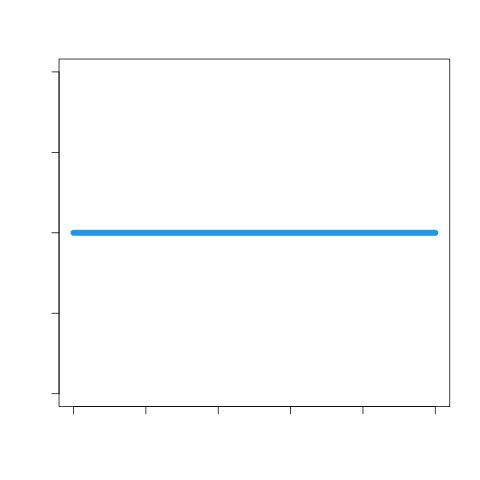
\includegraphics[width=.18\textwidth]{\fignet/FigMotifsBEDD-dist-h10} \end{tabular} &
    \begin{tabular}{c} 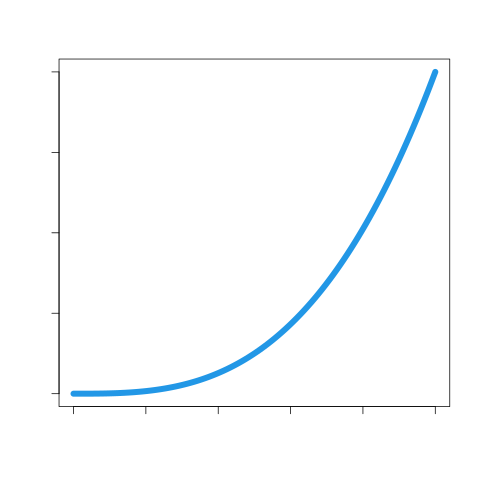
\includegraphics[width=.18\textwidth]{\fignet/FigMotifsBEDD-dist-h40} \end{tabular} \\
    \begin{tabular}{c} $g_0(u) =$ \end{tabular} &
    \begin{tabular}{c} 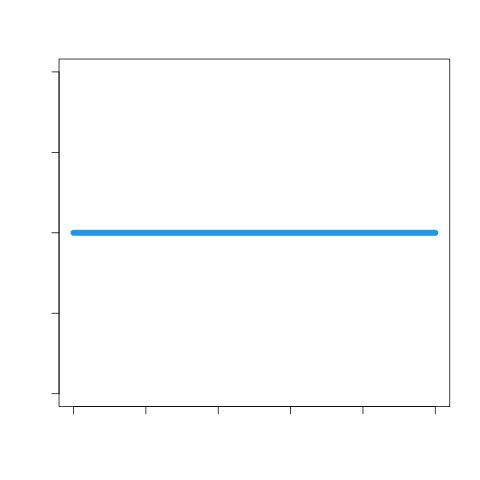
\includegraphics[width=.18\textwidth]{\fignet/FigMotifsBEDD-dist-g10} \end{tabular} &
    \begin{tabular}{c} 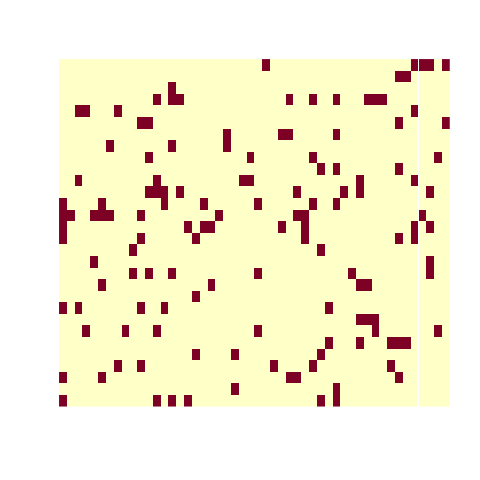
\includegraphics[width=.18\textwidth]{\fignet/FigMotifsBEDD-adj-g10-h10} \end{tabular} &
    \begin{tabular}{c} 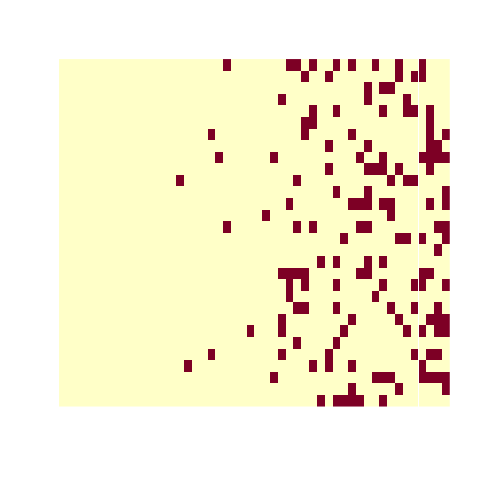
\includegraphics[width=.18\textwidth]{\fignet/FigMotifsBEDD-adj-g10-h40} \end{tabular} \\
    \begin{tabular}{c} $g(u) =$ \end{tabular} &
    \begin{tabular}{c} 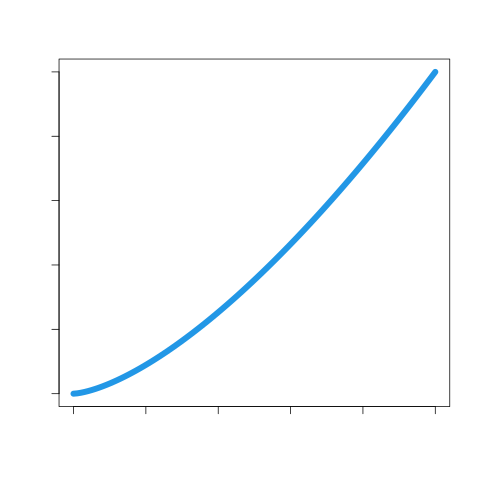
\includegraphics[width=.18\textwidth]{\fignet/FigMotifsBEDD-dist-g25} \end{tabular} &
    \begin{tabular}{c} 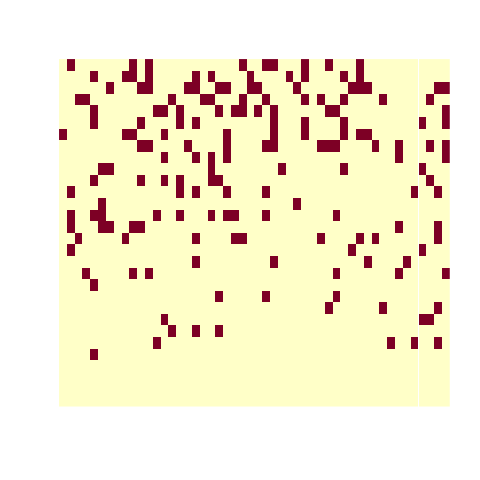
\includegraphics[width=.18\textwidth]{\fignet/FigMotifsBEDD-adj-g25-h10} \end{tabular} &
    \begin{tabular}{c} 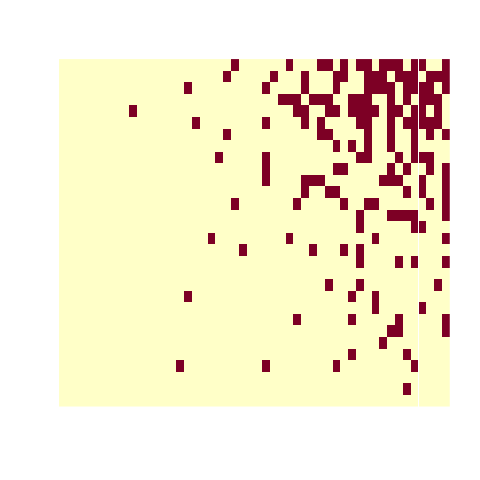
\includegraphics[width=.18\textwidth]{\fignet/FigMotifsBEDD-adj-g25-h40} \end{tabular} \\
  \end{tabular}
  
}

%==================================================================
\frame{\frametitle{Properties of the \BEDD model}

  \paragraph{Assumptions.}
  \begin{itemize}
    \setlength{\itemsep}{.75\baselineskip}
    \item No preferred or avoided specific connexion
    \item \emphase{Graph-exchangeable} model: pollinators can be permuted and plants can be permuted
  \end{itemize}
  
  \bigskip \bigskip \pause
  \paragraph{Properties.}
  \begin{itemize}
    \setlength{\itemsep}{.75\baselineskip}
    \item Expected degree for pollinator $i$ given $U_i$ : $n \; \rho \; g(U_i)$.
    \item Expected degree for plant $j$ given $V_j$ : $m \; \rho \; h(V_j)$.
    \item 'Nested' structure by construction
  \end{itemize}
  
  \bigskip \bigskip \pause
  \paragraph{Sufficient statistics} to fit \BEDD: 
  \begin{itemize}
    \setlength{\itemsep}{.75\baselineskip}
    \item Pollinator degrees + plant degrees
    \item or, equivalently, (single edge, top, bottom) star frequencies
  \end{itemize}

  }

%==================================================================
%==================================================================
\subsection{Motif count distribution}
%==================================================================
\frame{\frametitle{Counting motifs}

  \hspace{-.05\textwidth}
  \begin{tabular}{ll}
    \begin{tabular}{p{.4\textwidth}}
      \paragraph{Number of 'positions'.}
      \begin{itemize}
       \item Choose $p$ nodes among $m$
       \item Choose $q$ nodes among $n$
       \item Try all {\sl automorphisms} 
      \end{itemize}
      $$
      c_s := 
      \left(\begin{array}{c}m \\ p\end{array}\right)
      \times \left(\begin{array}{c}n \\ q\end{array}\right)
      \times r_s
      $$ 
      ~ \\ ~ \\
    \end{tabular}
    & \pause
    \begin{tabular}{p{.5\textwidth}}
      \paragraph{Automorphisms=} non-redundant permutations \\
      \includegraphics[width=.1\textwidth]{\fignet/FigMotifsBEDD-motif9-automorphism1}
      \includegraphics[width=.1\textwidth]{\fignet/FigMotifsBEDD-motif9-automorphism2}
      \includegraphics[width=.1\textwidth]{\fignet/FigMotifsBEDD-motif9-automorphism3} \\
      \includegraphics[width=.1\textwidth]{\fignet/FigMotifsBEDD-motif9-automorphism4}
      \includegraphics[width=.1\textwidth]{\fignet/FigMotifsBEDD-motif9-automorphism5}
      \includegraphics[width=.1\textwidth]{\fignet/FigMotifsBEDD-motif9-automorphism6} 
    \end{tabular} 
  \end{tabular}
  
  \bigskip \bigskip \pause
  \paragraph{Motif count.} Try all positions $\alpha = 1, \dots c_s$, define 
  $$
  Y_{s\alpha} = 1 \text{ if match,} \qquad 0 \text{ otherwise},
  $$
  then count the number of matches:
  $$
  N_s = \sum_\alpha Y_{s\alpha}
  $$
  \ra \emphase{Motif frequency}: $F_s := N_s / c_s$
  
}

% %==================================================================
% \frame{\frametitle{Motif probability}
% 
%   \paragraph{Occurrence probability $\overline{\phi}_s = \Pbb\{Y_{s\alpha} = 1\}$.} Under the B-EDD model \refer{OLR22}:
%   \begin{align*}
%     \overline{\phi}_s 
%     & :=
%     \Pbb_{\BEDD}\left(
%     \includegraphics[width=.06\textwidth, trim=100 200 100 0]{\fignet/FigMotifsBEDD-motif9} 
%     \right)
%     \; = \; 
%     \frac{
%     \onslide+<2->{
%       \overset{\text{top stars}}{\overbrace{
%       \Pbb\left(\includegraphics[width=.05\textwidth, trim=100 200 100 0]{\fignet/FigMotifsBEDD-motif9-top1}\right) % \times 
%       \Pbb\left(\includegraphics[width=.05\textwidth, trim=100 200 100 0]{\fignet/FigMotifsBEDD-motif9-top1}\right) % \times 
%       \Pbb\left(\includegraphics[width=.05\textwidth, trim=100 200 100 0]{\fignet/FigMotifsBEDD-motif9-top2}\right)   }}
%     }
%     \onslide+<3->{
%       \times
%       \overset{\text{bottom stars}}{\overbrace{
%       \Pbb\left(\includegraphics[width=.05\textwidth, trim=100 200 100 0]{\fignet/FigMotifsBEDD-motif9-bottom1}\right) % \times
%       \Pbb\left(\includegraphics[width=.05\textwidth, trim=100 200 100 0]{\fignet/FigMotifsBEDD-motif9-bottom3}\right)
%       }}
%     }
%     }{
%     \onslide+<4->{
%       \underset{\text{edges}}{\underbrace{
%       \left(\Pbb\left(\includegraphics[width=.05\textwidth, trim=100 200 100 0]{\fignet/FigMotifsBEDD-motif9-top1}\right)\right)^4
%       }}
%     }
%     } 
%     \\
%     \onslide+<5->{
%     & =
%     \frac{\left(\phi_1^2 \phi_2\right) \left(\phi_1 \phi_4\right)}{\left(\phi_1\right)^4}
%     \qquad =
%     \frac{\phi_2 \phi_4}{\phi_1}
%     }
%   \end{align*}
% 
%   \onslide+<6->{\bigskip \bigskip 
%   \paragraph{Estimated probability.} 
%   $$
%   \overline{\phi}_s := \frac{\phi_2 \phi_4}{\phi_1}
%   \qquad \rightarrow \qquad 
%   \overline{F}_s := \frac{F_2 F_4}{F_1}
%   $$
%   where $F_1$, $F_2$, $F_4 =$ observed frequencies of  edges, top stars and bottom stars.
%   }
% }

%==================================================================
\frame{\frametitle{Motif probability}

  \label{sec:motifProba}
  \paragraph{Occurrence probability $\overline{\phi}_s = \Pbb\{Y_{s\alpha} = 1\}$.} Under the B-EDD model \refer{OLR22}:
  \begin{align*}
    \left(\includegraphics[width=.06\textwidth, trim=100 200 100 0]{\fignet/FigMotifsBEDD-motif9}\right) 
    & = \; 
    \frac{
    \onslide+<2->{
      \overset{\text{top stars}}{\overbrace{
      \left(\includegraphics[width=.05\textwidth, trim=100 200 100 0]{\fignet/FigMotifsBEDD-motif9-top1}\right) % \times 
      \left(\includegraphics[width=.05\textwidth, trim=100 200 100 0]{\fignet/FigMotifsBEDD-motif9-top1}\right) % \times 
      \left(\includegraphics[width=.05\textwidth, trim=100 200 100 0]{\fignet/FigMotifsBEDD-motif9-top2}\right)   }}
    }
    \onslide+<3->{
      \quad
      \overset{\text{bottom stars}}{\overbrace{
      \left(\includegraphics[width=.05\textwidth, trim=100 200 100 0]{\fignet/FigMotifsBEDD-motif9-bottom1}\right) % \times
      \left(\includegraphics[width=.05\textwidth, trim=100 200 100 0]{\fignet/FigMotifsBEDD-motif9-bottom3}\right)
      }}
    }
    }{
    \onslide+<4->{
      \underset{\text{edges}}{\underbrace{
      \left(\includegraphics[width=.05\textwidth, trim=100 200 100 0]{\fignet/FigMotifsBEDD-motif9-top1}\right)^4
      }}
    }
    } 
    \\
    \onslide+<5->{
    \overline{\phi}_s 
    =
    \Pbb_{\BEDD}\left(
    \includegraphics[width=.06\textwidth, trim=100 200 100 0]{\fignet/FigMotifsBEDD-motif9} 
    \right)
    & = \;
    \frac{\left(\phi_1^2 \phi_2\right) \left(\phi_1 \phi_4\right)}{\left(\phi_1\right)^4}
    \qquad =
    \frac{\phi_2 \phi_4}{\phi_1}
    \qquad \goto{sec:motifList}
    }
  \end{align*}

  \onslide+<6->{\bigskip 
  \paragraph{Estimated probability $\overline{F}_s$.} 
  $$
  \overline{\phi}_s := \frac{\phi_2 \phi_4}{\phi_1}
  \qquad \rightarrow \qquad 
  \overline{F}_s := \frac{F_2 F_4}{F_1}
  $$
  where $F_1$, $F_2$, $F_4 =$ observed frequencies of  edges, top stars and bottom stars.
  }
}

%==================================================================
\frame{\frametitle{Moments of the count} \label{sec:motifMoments}

  \begin{itemize}
  \setlength{\itemsep}{.75\baselineskip}
  \item \emphase{Number of positions:} $c_s$ \qquad (frequency: $F_s = N_s \,/\, c_s$)
  \item \emphase{Mean:} $\Esp_{\BEDD}(N_s) = c_s \times \overline{\phi}_s$ 
  \item \pause \emphase{Variance:} Same game, requires to evaluate $\displaystyle{\Esp_{\BEDD}(N_s ^2) = \Esp_{\BEDD}\left(\sum_\alpha Y_{s\alpha} \right)^2}$ \\
  \ra Need to account for overlap between positions ({\sl super-motifs}: \refer{PDK08} \goto{back:superMotifs}) 
  $$
  \includegraphics[width=.8\textwidth, trim=0 25 0 0, clip=]{\fignet/OLR22-EJS-Fig2}
  $$ 
  \ra Compute the respective expected count in the way as for regular motifs \\ ~
  \item \pause \emphase{Covariance:} Same game to compute $\Cov(N_s, N_{s'})$
  \item \pause \emphase{Asymptotic normality:} \goto{back:motifDistrib} \goto{back:asymNormality}
  $
  (N_s - \overline{N}_s) \left/ \sqrt{\widehat{\Var}(N_s)} \right. \quad \overset{m, n \rightarrow \infty}{\longrightarrow} \quad \Ncal(0, 1)
  $ 
  \end{itemize}

}

%==================================================================
\frame{\frametitle{Distribution of the count}

  \paragraph{Asymptotic normality for non-star motifs.} Under \BEDD (and sparsity conditions):
  $$
  (F_s - \overline{F}_s) \left/ \sqrt{\widehat{\Var}(F_s)} \right. \quad \overset{m, n \rightarrow \infty}{\longrightarrow} \quad \Ncal(0, 1)
  $$
  Proof \refer{OLR22}: 
  \begin{equation*}
    \text{decompose} \qquad
   F_s - \overline{F}_s 
   = \underset{\text{random fluctuations}}{\underbrace{(F_s - \phi_s)}} 
   + \underset{\text{null under \BEDD}}{\underbrace{(\phi_s - \overline{\phi}_s)}}  
   + \underset{\text{estimation error } \rightarrow 0}{\underbrace{(\overline{\phi}_s - \overline{F}_s)}}, 
  \end{equation*}
  + construct a counting martingale for $F_s - \phi_s$  \refer{GaL17b}.
  
  \bigskip \bigskip \pause
  \paragraph{Consequence.} We know 
  \begin{itemize}
    \item the expected behavior (mean, variance, distribution) of any motif count 
    \item under the BEDD model (= 'null model').
  \end{itemize}
}

%==================================================================
%==================================================================
\subsection{(Distance-based) network comparison}
% \frame{\frametitle{Outline} \tableofcontents[currentsubsection]}
%==================================================================
\frame{\frametitle{Comparing network imbalances}

  \bigskip
  \paragraph{Question.} Do network $A$ and $B$ share the same imbalance for pollinators?
  
  \bigskip \pause
  \paragraph{Statistical test.} 
  \begin{itemize}
    \item Assume $A \sim BEDD(\rho^A, g^A, h^A)$ and $B \sim BEDD(\rho^B, g^B, h^B)$
    $$
    H_0 = \{g^A = g^B\}
    $$
    \item For motif $s$, evaluate $\widehat{\Esp}_{\widehat{\rho}^A, \emphase{\widehat{g}^B}, \widehat{g}^A}(N^A_s)$ and $\widehat{\Esp}_{\widehat{\rho}^B, \emphase{\widehat{g}^A}, \widehat{g}^B}(N^B_s)$ and compare 
    $$
    W^{\textcolor{gray}{(g)}}_s\textcolor{gray}{(A, B)} = \frac{(N_s^A - \widehat{\Esp}_0(N_s^A)) - (N_s^B - \widehat{\Esp}_0(N_s^B))}{\sqrt{\widehat{\Var}_0(N^A_s) + \widehat{\Var}_0(N^B_s)}}
    $$ 
    with $\Ncal(0, 1)$
  \end{itemize}

  
  \bigskip \pause
  \paragraph{Example.} (no significant difference) 
  $$
  \begin{array}{c}
    \includegraphics[width=.8\textwidth, trim=0 50 0 0, clip=]{\fignet/OLR22-EJS-Tab4} \\ 
    \includegraphics[width=.8\textwidth, trim=0 0 0 90, clip=]{\fignet/OLR22-EJS-Tab4}   
  \end{array}
  $$

}

% %==================================================================
% %==================================================================
% \subsection{Distance-based network comparison}
% % \frame{\frametitle{Outline} \tableofcontents[currentsubsection]}
%==================================================================
\frame{\frametitle{Plant-pollinator networks in space \& time}
  
  \paragraph{Questions.} Does the structure of plant (herbaceous species) pollinator (native wild bees and hoverflies) network differ\footnote{Joint work with Natasha de Manincor \& Fran\c{c}ois Massol + Sarah Ouadah \& Pierre Latouche}: 
  \begin{itemize}
    \item along the environmental gradient?
    \item across sites within the season?
  \end{itemize}  
  
  \bigskip \bigskip \pause
  \paragraph{Dataset.}
  \begin{itemize}
    \item 6 sites: 3 regions (Hauts-de-France, Normandie and Occitanie) $\times$ 2 sites per region
    \item 2 years (2016, 2017)
    \item 7 months (April to October) per year
  \end{itemize}
  $$
  \to \quad N=82 \text{ networks}, \quad [4, 39] \text{ plants}, \quad [8, 80] \text{ insects}
  $$
    
  \bigskip \bigskip \pause
  \paragraph{Approach.} Define a motif-based distance between each pair of networks.
%   \bigskip ~

}

%==================================================================
\frame{\frametitle{Distance-based network comparison}

  \begin{tabular}{ll}
    \hspace{-.04\textwidth}
    \begin{tabular}{p{.55\textwidth}}
      \paragraph{Network distance.} For a pair of networks $(A, B)$
      \begin{itemize}
        \item for a given comparison (e.g. insect imbalance): 
        $$H_0^{(g)} = \{g^A = g^B\},$$ 
        \item for a given motif $s$: test statistic $W_s^{(g)}$, 
        \item define the 'distances': 
        $$
        D^{(g)}(A, B) = \sqrt{\sum_s \left(W_s^{(g)}\right)^2}
        $$
      \end{itemize}
    \end{tabular}
    &
    \pause
    \hspace{-.05\textwidth}
    \begin{tabular}{p{.45\textwidth}}
      \paragraph{Distance matrix:} \\
%       $$
      \includegraphics[width=.45\textwidth, trim=0 10 20 50, clip=]{\fignatA/All_NatashaBinNetList-stat3-distMat}
%       $$
    \end{tabular} 
  \end{tabular}

  \bigskip \bigskip \pause
  The same for 
  \begin{itemize}
    \item plant imbalance: $H_0^{(h)} = \{h^A = h^B\}$ $\to W_s^{(h)}$ $\to D^{(h)}(A, B)$ 
    \item both imbalance: $H_0^{(gh)} = \{g^A = g^B, h^A = h^B\}$ $\to W_s^{(gh)}$ $\to D^{(gh)}(A, B)$ 
  \end{itemize}
}

%==================================================================
\frame{\frametitle{Distance-based analysis of variance ('Adonis')} \label{sec:adonis}

  \bigskip
  \paragraph{Data at hand.} $N$ networks ($A = 1, \dots N$)
  \begin{itemize}
    \setlength{\itemsep}{.75\baselineskip}
    \item network covariates: e.g. region, year, month, \dots
    \item distance matrix $D = [D(A, B)]$ for all pairs of networks
  \end{itemize}

  \bigskip \bigskip \pause
  \paragraph{Analysis of variance for distance matrices \refer{And01}.} Briefly speaking:
  \begin{itemize}
    \setlength{\itemsep}{.75\baselineskip}
    \item Think of the regular linear model (regression, analysis of variance)
    \item Do as if the distance was computed on pseudo variable rules by a linear model
    \item 'Model':
    \begin{align*}
    D(A, B) = f(& \text{region}_A, \text{region}_B, \text{month}_A, \text{month}_B, \\
    & (\text{region*month})_A, (\text{region*month})_B, \dots)
    \end{align*}
    \item Compute a pseudo $F$ statistics for each effect of interest
    \item Assess significance using permutation tests.
  \end{itemize}
  
  \medskip
  (see \refer{McA01,ZaS06} \goto{back:adonis}, \url{vegan} R package --\url{adonis2}--)

}

%==================================================================
\frame{\frametitle{Results} \label{sec:adonisResults}
  
  \paragraph{Insect imbalance $D^{(g)}$.}
  $$\small{
  \begin{tabular}{l|rrrrr}
    & Df & Sum Of Sqs & $R^2$ & F & Pr(\>F) \\ 
\hline
\emphase{InsectNb} & 1 & 69.9 & 0.2595 & 42.69 & \emphase{1e-05} \\ 
\emphase{PlantNb} & 1 & 31.17 & 0.1157 & 19.04 & \emphase{1e-05} \\ 
Year & 1 & 2.66 & 0.0099 & 1.62 & 0.22212 \\ 
\emphase{Month} & 6 & 24.8 & 0.092 & 2.52 & \emphase{0.00959} \\ 
\emphase{Region} & 2 & 8.67 & 0.0322 & 2.65 & \emphase{0.04531} \\ 
Year:Month & 6 & 4.81 & 0.0179 & 0.49 & 0.88756 \\ 
Year:Region & 2 & 5.51 & 0.0204 & 1.68 & 0.1787 \\ 
{\bf Month:Region} & 12 & 32.41 & 0.1203 & 1.65 & {\bf 0.06346} \\ 
Year:Month:Region & 12 & 27.26 & 0.1012 & 1.39 & 0.15884 \\ 
Residual & 38 & 62.22 & 0.2309 & &  \\ 
Total & 81 & 269.42 & 1 & & 

  \end{tabular}
  }$$

  \begin{itemize}
    \setlength{\itemsep}{.75\baselineskip}
    \item \pause Because of small network sizes, need to correct for the number of insects and plants \goto{back:adonisNull}
    \item \pause Significant effect of the region and the month, indicating change of the insect imbalance both in space and time
    \item \pause The pattern is conserved from year to the next (not year effect)
    \item \pause No effect is found for the plant imbalance distance $D^{(h)}$ \goto{back:adonisOther}
  \end{itemize}

}

